\section{Structured Flow Matching}
\label{sec:methods}

This section develops StructFlow bottom-up: flow-matching primitives, then block-triangular velocity fields and what they preserve and make tractable, then the compiler. Figure~\ref{fig:dual-flow} previews the pipeline.

\begin{figure*}[hbt!]
    \centering
    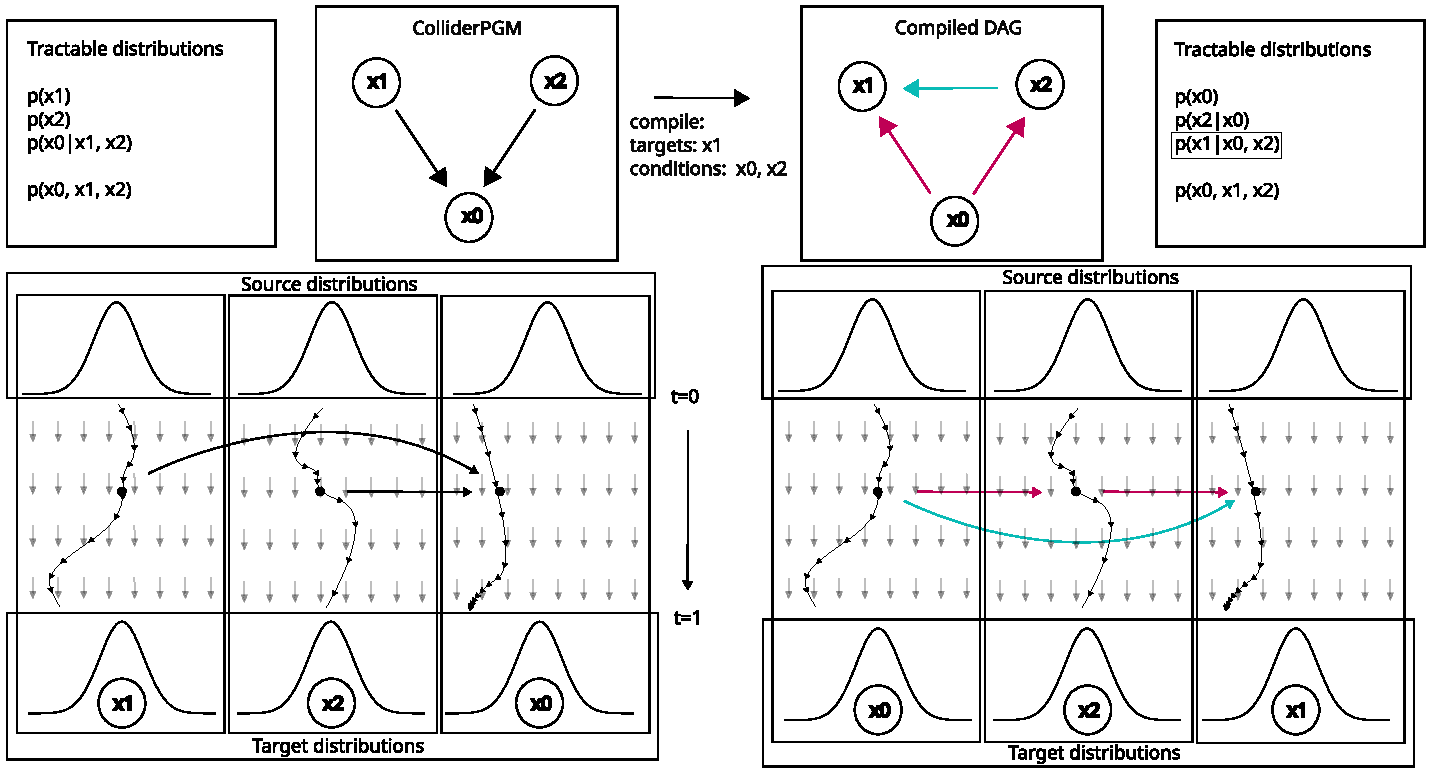
\includegraphics[width=\textwidth]{images/collider-pgm-dual.pdf}
    \caption{\textbf{The StructFlow Pipeline.} Given a causal graph (top, second from left) and an inference query $p(x_1 \mid x_0, x_2)$, StructFlow compiles the graph into a flow architecture. 1. The graph is \textbf{moralized}: because the common effect $x_0$ is observed, its causes $x_1$ and $x_2$ become dependent (``explaining away''), so the compiled DAG gains the teal edge $x_2 \to x_1$. 2. The blocks are ordered with the conditions first ($x_0$, then $x_2$) and the target $x_1$ last, so each block's flow is conditioned on the variables it depends on. The boxes on either side list the distributions each structure makes tractable; below each DAG is its flow, one block per variable, transporting noise (top) to data (bottom).}
    \label{fig:dual-flow}
\end{figure*}

\subsection{Flow Matching Primitives}
Continuous Normalizing Flows (CNFs) transport a simple base density $p_0$ (e.g., $\mathcal{N}(0, I)$) to a complex target $p_1$ along a time-dependent vector field $v_t: \mathbb{R}^d \times [0,1] \to \mathbb{R}^d$: the flow $\phi_t$ solves $\frac{d}{dt}\phi_t(y) = v_t(\phi_t(y))$ with $\phi_0(y) = y$, and integrating from $t=0$ to $1$ carries a sample $y_0 \sim p_0$ to $y_1 = \phi_1(y_0) \sim p_1$. \textbf{Flow Matching} \citep{lipman2022flow} trains the parameterized field $v_t^\phi$ without simulating this ODE, by regressing onto a target conditional field $u_t$ that generates a chosen probability path:
\begin{equation}
    \mathcal{L}(\phi) = \mathbb{E}_{t \sim \mathcal{U}(0,1),\, y_1 \sim p_1,\, y_0 \sim p_0} \left[ \left\| v_t^\phi(y_t) - u_t(y_t \mid y_0, y_1) \right\|^2 \right],
\end{equation}
where, for the linear interpolant, $y_t = (1-t)y_0 + ty_1$ and $u_t(y_t \mid y_0, y_1) = y_1 - y_0$.

\subsection{Block-Triangular Architectures}
\label{sec:block-triangular}

We define a \textbf{Block-Triangular Flow} as a CNF whose velocity field respects a DAG structure $\mathcal{G}$. Let the state $y \in \mathbb{R}^d$ be partitioned into $K$ disjoint blocks $y = [y^{(1)}, \dots, y^{(K)}]$, ordered according to a topological sort of $\mathcal{G}$. The velocity field decomposes as:
\begin{equation}
\frac{d y^{(k)}_t}{dt} = v^{(k)}_\phi\bigl(y^{(k)}_t, \mathrm{Pa}_\mathcal{G}(y^{(k)})_t, t\bigr), \quad k = 1, \dots, K
\end{equation}
where $\mathrm{Pa}_\mathcal{G}(y^{(k)}) \subseteq \{y^{(1)}, \dots, y^{(k-1)}\}$ denotes the parents of block $k$ in the DAG $\mathcal{G}$.

\textbf{Example (Chain).} For $X \to Y \to Z$, block $Z$'s velocity sees $Y$ but not $X$, respecting $Z \perp X \mid Y$.

This constraint ensures the Jacobian $J = \frac{\partial \phi_1(y_0)}{\partial y_0}$ is block lower-triangular, with the log-determinant decomposing as $\log|J| = \sum_{k=1}^K \log|J^{(kk)}|$. This structure enables tractable marginal densities and efficient conditional sampling by fixing parent trajectories. However, this tractability is \emph{asymmetric} and depends strictly on the variable ordering.

The block-triangular structure is realized purely through the connectivity of the velocity network, and it is preserved by the flow dynamics:

\begin{proposition}[Structural Preservation]
\label{prop:structural-preservation}
\rev{Assume velocity fields regular enough for unique, continuously differentiable flows (existence--uniqueness and spatial Lipschitzness, as in \citet{jeong_conditional_2025}, Assumptions~1--2). Parameterize the velocity through a denoiser $\hat{\eta}_1$ under the linear interpolant $y_t = (1-t)y_0 + t y_1$. (i)~If the $k$-th block depends only on the prefix, $\hat{\eta}_1^{(k)}(y, t) = \mathrm{NN}^{(k)}(y^{(1)}, \dots, y^{(k)}, t)$, the induced velocity and flow map are block-triangular and the learned density factorizes autoregressively along the ordering. (ii)~If block $k$ depends only on its graph parents, the jointly-integrated flow map depends on the base noise of $\{k\} \cup \mathrm{Anc}(k)$, refining the conditionals to ancestor sets---ancestral, not yet parental, sparsity. (iii)~Sequential integration with parents resolved to their final values (static conditioning, the causal-mode sampler) sharpens this to the Markov factorization $p(y) = \prod_k p\bigl(y^{(k)} \mid y^{(\mathrm{Pa}(k))}\bigr)$ of $\mathcal{G}$.}
\end{proposition}

This is the architectural guarantee underlying StructFlow (proof in Appendix~\ref{app:proof}): constraining \emph{which inputs each block of the network sees} makes the transport respect the graph, \rev{with the exact granularity---prefix, ancestral, or parental---set by the masking and the integration schedule}. The same structure, however, makes density computation \emph{order-dependent}:

\begin{theorem}[Asymmetry of Marginalization]
\label{thm:marginalization}
In a Block-Triangular Flow with ordering $y^{(1)} \to \cdots \to y^{(K)}$, call the marginal $\log p(y_S)$ of a subset $S$ \emph{directly tractable} if it can be evaluated by the change-of-variables formula restricted to $S$ (a single pass, with no integration over the remaining variables). If $S$ is \emph{ancestrally closed}---contains all parents, and hence all ancestors, of each of its members---then $\log p(y_S)$ is directly tractable; a topological \emph{prefix} $S = \{1, \dots, k\}$ is the canonical such set, and is the case used by our compiler. \rev{Conversely, if $S$ is not ancestrally closed, the restricted formula is invalid for any flow whose missing-ancestor dependencies are functionally non-degenerate (the generic case), and exact evaluation requires marginalizing them out, which is intractable in general.}
\end{theorem}

\textbf{Implication} (proof in Appendix~\ref{app:proof}). This explains why a single fixed architecture cannot efficiently serve both tasks: a causal model ordered $X \to Y$ computes $p(X)$ and $p(X,Y)$ efficiently but must marginalize over $X$ for $p(Y)$, whereas efficient inference $p(X \mid Y)$ needs $Y$ ahead of $X$---a task-specific re-ordering. \rev{Corollary~\ref{cor:query-family} (appendix) makes the supported family explicit: a compilation \emph{samples} $p(T \mid C)$ for every condition-prefix $C$ and arbitrary targets $T$, marginalizing nuisance variables by sampling; \emph{densities} additionally require ancestral closure.}

\subsection{StructFlow: Structural Flow Alignment}
\label{sec:structflow}

A Probabilistic Graphical Model defines a generative factorization of a joint distribution $p(y) = \prod_{k} p(y^{(k)} \mid \mathrm{Pa}(y^{(k)}))$ via a DAG $\mathcal{G}$. We introduce \textbf{StructFlow} (Structural Flow Alignment), an algorithm that translates the abstract graph $\mathcal{G}$ into a concrete block-triangular flow architecture tailored to a specific probabilistic query. Depending on the desired capability, StructFlow produces one of two distinct model artifacts (each trained separately).

Three standard assumptions delimit the queries StructFlow can answer correctly.

\begin{assumption}[Standard causal assumptions]
\label{ass:standard}
(i) \emph{Causal sufficiency:} $\mathcal{G}$ contains no unobserved confounders---every common cause of two variables in $\mathcal{G}$ is itself a node of $\mathcal{G}$. (ii) \emph{Markov condition:} the data distribution factorizes according to $\mathcal{G}$. (iii) \emph{Faithfulness:} every conditional independence in the data distribution is entailed by d-separation in $\mathcal{G}$.
\end{assumption}

Parts (i)--(ii) let the causal-alignment model identify interventional distributions, so that fixing parents in the flow corresponds to a $\mathrm{do}(\cdot)$ operation (Theorem~\ref{thm:level2}). Faithfulness (iii) is used by the inference compiler to prune a candidate dependency whenever the corresponding variables are d-separated, making the compiled inference graph both \emph{sufficient} (no posterior dependency is missed) and \emph{minimal}. We assume $\mathcal{G}$ is known; structure discovery is orthogonal (Section~\ref{sec:future_work}). Counterfactual queries require an additional identifiability condition (Remark~\ref{rem:cf-identifiability}).

\subsubsection{Causal Alignment}
When the goal is mechanistic simulation or causal reasoning, StructFlow preserves the DAG structure directly. The flow blocks are ordered according to a topological sort of $\mathcal{G}$ (roots $\to$ leaves), and each block's velocity field receives inputs only from its DAG parents:
\begin{equation}
    v^{(k)}_\phi(y^{(k)}_t, \mathrm{Pa}_\mathcal{G}(y^{(k)})_t, t)
\end{equation}
Because this structure mirrors the causal mechanisms (respecting the Principle of Independent Mechanisms \citep{Peters2017}), the resulting flow enables interventional queries $p(y \mid \mathrm{do}(x))$ by fixing parent values, and counterfactual queries via flow inversion (Section~\ref{sec:counterfactuals}).

This is more than an analogy: with static conditioning each block reads its parents only through their \emph{terminal} values, so the flow map is literally a system of structural equations driven by independent noise.

\begin{lemma}[The causally-aligned flow is an SCM]
\label{lem:mech-main}
Let $\phi_1$ be the flow map of a causally-aligned StructFlow with static conditioning and a spatially Lipschitz velocity field. Then there exist maps $G_1,\dots,G_K$ such that, for $u \sim p_0$ and
$\hat x = \phi_1(u)$,
\begin{equation}
    \hat x^{(k)} = G_k\bigl(\hat x^{(\mathrm{Pa}_\mathcal{G}(k))},\, u_k\bigr),
    \qquad k = 1,\dots,K,
\end{equation}
with $u_1,\dots,u_K$ mutually independent and each $G_k$ invertible in $u_k$ at fixed parent values, pushing the base block onto the learned conditional $\hat p\bigl(x^{(k)} \mid x^{(\mathrm{Pa}(k))}\bigr)$.
\end{lemma}

This is the $K$-block generalization of Lemma~1 of \citet{jeong_conditional_2025}, and it
licenses the causal reading of the architecture: clamping a block replaces a mechanism rather than conditioning on it. Three consequences follow, proved in
Appendix~\ref{app:hierarchy}: recovering the observational joint recovers \emph{every}
interventional distribution, for arbitrary structural equations, with the interventional
density available in one pass (Theorem~\ref{thm:level2},
Corollary~\ref{cor:interventional-density}); counterfactuals are recovered exactly at the flow-matching optimum whenever each mechanism is monotone coordinate-wise in independent noise or additive, which includes all linear structural equations and our synthetic benchmarks (Theorem~\ref{thm:level3}); and none of this identifies the graph itself---in the linear--Gaussian case every Markov-equivalent DAG
attains the same optimal flow-matching loss while giving different causal answers
(Proposition~\ref{prop:mec}). These guarantees are for static conditioning. Under dynamic conditioning a block reads its ancestors' trajectories, so the learned flow is an SCM on the transitive closure of $\mathcal{G}$ (each parent set replaced by the ancestor set) rather than on $\mathcal{G}$; with the per-block coupling it still targets the correct conditionals, but we do not claim the mechanism-level guarantees for it (Remark~\ref{rem:static-dynamic-equal}).

\subsubsection{Inference Alignment}
When the goal is amortized posterior inference $p(\Theta \mid Y)$ where $\Theta$ are latent variables and $Y$ are observations, StructFlow must address two challenges: \emph{ordering}---by Theorem~\ref{thm:marginalization}, the observations $Y$ must precede the targets $\Theta$ for tractable conditional evaluation---and \emph{posterior dependencies}---the posterior can be \emph{denser} than the prior (at a collider $X_1 \to Y \leftarrow X_2$ with $X_1 \perp X_2$ marginally, observing $Y$ induces $X_1 \not\perp X_2 \mid Y$, a correlation the original DAG has no edge to carry). The compilation pipeline for inference mode consists of three steps:
\begin{enumerate}
    \item \textbf{Moralization:} Connect all pairs of variables sharing a common child in $\mathcal{G}$, then drop edge directions. The posterior is not a causal object---the dependencies conditioning induces (such as the collider coupling above) are symmetric constraints, which the moral graph is guaranteed to contain \citep{Koller2009}.

    \item \textbf{Re-ordering:} Compute a valid ordering where all observations $Y$ precede all targets $\Theta$---not a heuristic but the tractability requirement of Theorem~\ref{thm:marginalization} (within each group we use reverse topological order, which tends to yield sparser parent sets after pruning).

    \item \textbf{Dependency Pruning:} For each target $\theta_k$ in the computed order, determine its minimal parent set using d-separation:
    \begin{equation}
        j \in \mathrm{Pa}_{\text{flow}}(\theta_k) \iff \theta_k \not\perp_d z_j \mid \{z_1, \dots, z_{k-1}\} \setminus \{z_j\},
    \end{equation}
    where $z_1, \dots, z_{k-1}$ precede $\theta_k$. The first two steps overshoot (a complete graph always suffices); the d-separation test removes every dependency the graph refutes, restoring the sparsity that acts as the inductive bias of Appendix~\ref{sec:sample-efficiency}.
\end{enumerate}

The conditioning mechanisms of Section~\ref{sec:conditioning} then operate on this \emph{compiled} graph---the moralized, re-ordered, pruned structure---not on the original DAG. \rev{The two steps divide the work: the dependency set is constructed \emph{entirely} by the d-separation step---explaining-away dependencies between co-parents appear under every conditions-first ordering---while moralization only guides the ordering, toward sparser compiled structures (ablation in Appendix~\ref{app:ordering-ablation}).} Appendix~\ref{app:worked-example} walks the full pipeline through a dense four-node example, including a query for which conditioning and intervening differ, and Appendix~\ref{app:algorithms} gives the explicit algorithms.

\paragraph{One engine per ordering, not per query.} Compilation is specific to a query \emph{class}: a single inference-aligned flow with ordering $[Y, \Theta]$ answers every query whose conditioning set is a prefix of that ordering (the tractable family of Theorem~\ref{thm:marginalization}), for any observed values, without retraining; only a different observation/target split triggers a new compilation and training run. Compilation itself is negligible---$O(K^2)$ d-separation tests, each linear in the size of the graph \citep{Koller2009}---so the dominant cost is flow-matching training, the same cost paid by any CNF of comparable connectivity.

\subsection{Conditioning Mechanisms}
\label{sec:conditioning}

Given a block-triangular flow with ordering $[Y, \Theta]$ (observations first, targets second), we must specify how the target velocity field $v^{(\Theta)}_\phi$---the components governing the evolution of $\Theta$---receives information from the conditioning variables $Y$. We implement two strategies: static conditioning, the standard construction in conditional CNFs and diffusion models (the condition enters as a fixed input), and dynamic conditioning, the recent alternative of \citet{jeong_conditional_2025}.

\paragraph{Static Conditioning.}
In static mode, conditioning variables are first integrated to completion, then their \emph{final values} $y_1 = \phi_1(y_0)$ are provided as fixed inputs to the target velocity field:
\begin{equation}
    \frac{\partial \theta_t}{\partial t} = v^{(\Theta)}_\phi(\theta_t, y_1, t)
\end{equation}
Sampling proceeds sequentially---one ODE solve per block, each block conditioned on the terminal values of its already-integrated parents---so a query with $K$ target blocks requires $K$ sequential solves (observed conditions are fixed values and need none).

\paragraph{Dynamic Conditioning.}
In dynamic mode, all variables are integrated \emph{simultaneously} in a single ODE solve. The target velocity field is conditioned on the \emph{time-evolving trajectory} of the conditioning variables:
\begin{equation}
    \frac{d\theta_t}{dt} = v^{(\Theta)}_\phi(\theta_t, y_t, t)
\end{equation}
where $y_t$ co-evolves with $\theta_t$. This requires the network to learn meaningful representations from partially-noised conditioning variables (at intermediate times $t < 1$), but enables a single parallel ODE integration for all variables. The two mechanisms are contrasted schematically in Appendix Figure~\ref{fig:static-v-dynamic-conditioning}.

\subsection{Counterfactual Inference}
\label{sec:counterfactuals}

Block-triangular flows enable counterfactual reasoning---given an observation $(x, y)$ from a causal model $X \to Y$, answering ``what would $Y$ have been if $X$ had been $x'$?'', formally $p(Y_{x'} \mid X{=}x, Y{=}y)$---via the Abduction-Action-Prediction framework \citep{Pearl2009} (illustrated in Appendix Figure~\ref{fig:counterfactual}). The flow's bijectivity recovers the noise $u$ that generated an observation under the learned model, which allows re-simulation under a hypothetical intervention:

\begin{enumerate}
    \item \textbf{Abduction:} Recover the noise by inverting the flow: integrate $\frac{dy_t}{dt} = -v_t(y_t)$ backward from $y_1 = y_{\text{obs}}$ to obtain $u = \phi_1^{-1}(y_{\text{obs}})$.
    \item \textbf{Action:} Realize $\mathrm{do}(X = x')$ by replacing the natural evolution of $X$ with a fixed trajectory: for static flows, set $x_1 = x'$; for dynamic flows, construct the full trajectory $x'_t$ by integrating backward from $x'$.
    \item \textbf{Prediction:} Integrate $\frac{d\theta_t}{dt} = v^{(\Theta)}_\phi(\theta_t, x'_t, t)$ forward from the \emph{original} noise, $\theta_0 = u_\Theta$, with the intervened variable fixed to its counterfactual trajectory.
\end{enumerate}

\begin{remark}[Counterfactual identifiability]
\label{rem:cf-identifiability}
Abduction recovers the noise $u = \phi_1^{-1}(y_{\mathrm{obs}})$ consistent with the observation \emph{under the learned model}, which is not necessarily the true exogenous noise of the data-generating process. Theorem~\ref{thm:level3} identifies
when the discrepancy is harmless: for a static flow at the flow-matching optimum, if each mechanism is monotone coordinate-wise in independent noise or additive (a class covering all linear structural equations and our synthetic benchmarks), the mismatch is a parent-independent reparameterization that cancels
between abduction and prediction, and the recovered counterfactual is exact. For multivariate blocks that are neither---such as the image block of Section~\ref{sec:colored-mnist}---the condition fails, and those counterfactuals
remain model-based estimates (Remark~\ref{rem:l3-limits}). All of this presumes the graph is
correct; that presumption is the binding one (Proposition~\ref{prop:mec}).
\end{remark}
